\documentclass{beamer}


\usepackage[no-math]{fontspec}
\usepackage{xunicode}
\usepackage{xltxtra}
\usepackage{tikz}
\usepackage{graphicx}
\usepackage{booktabs}
\usepackage{fontawesome}
\usepackage[normalem]{ulem}
\usepackage[mode=text]{siunitx}
\usepackage{hyperref}


% Beamer setup
\mode<presentation>
{
	\usetheme{OtagoPlain}
	\setbeamertemplate{navigation symbols}{}
}
\setbeamertemplate{footline}[frame number]


% TikZ setup
\usetikzlibrary{positioning}
% \usetikzlibrary{graphs}
% \usetikzlibrary{decorations.pathreplacing}
\usetikzlibrary{calc}
\usetikzlibrary{arrows.meta}
\usetikzlibrary{shapes.geometric}


% fontspec setup
\defaultfontfeatures{Mapping=tex-text}
\setmainfont{Minion Pro}
\setsansfont[Scale=MatchUppercase,BoldFont={Open Sans}]{Open Sans Light}
\setmonofont[Scale=MatchLowercase]{Letter Gothic 12 Pitch}


% graphicx setup
\graphicspath{{images/}}


% misc
\newcommand{\todo}[1]{\alert{\textbf{!!TODO!! [#1] !!}}}


% Draw a grid to aid TikZ picture drawing/debugging.
\newcommand{\DrawGridTikZ}[2]{%
	\begin{scope}[color=lightgray]
		\draw[thin,step=1mm]  (0.0,0.0)   grid (#1,#2);%
		\draw[thick,step=1cm] (-0.1,-0.1) grid (#1+0.1,#2+0.1);%
		\pgftext[top,at={\pgfxy(0.0,-0.2)}]{\tiny 0}%
		\pgftext[right,at={\pgfxy(-0.2,0.0)}]{\tiny 0}%
		\foreach \x in {1,...,#1} {\pgftext[top,at={\pgfxy(\x,-0.2)}]{\tiny\x}}%
		\foreach \y in {1,...,#2} {\pgftext[right,at={\pgfxy(-0.2,\y)}]{\tiny\y}}%
	\end{scope}
}


% Sometimes we want to put a comment in tiny text on the next line, but the default line skip
% will insert too much vertical space. Put a \tinyskip at the end of the line instead.
\def\tinyskip{\\[-0.33\baselineskip]}


% Bold-face text using the structure colour.
\newcommand<>{\structurebf}[1]{\structure#2{\textbf{#1}}}


% preamble
\title{Adventures in data wrangling}
\author{Nigel Stanger}
\date{July 20, 2018}


\begin{document}


%%%%%%%%%%%%%%%%%%%%%%%%%%%%%%%%%%%%%%%%%%%%%%%%%%%%%%%%%%%%%%%%%%%%%%%%%%%%%%%%


\setbeamertemplate{background canvas}{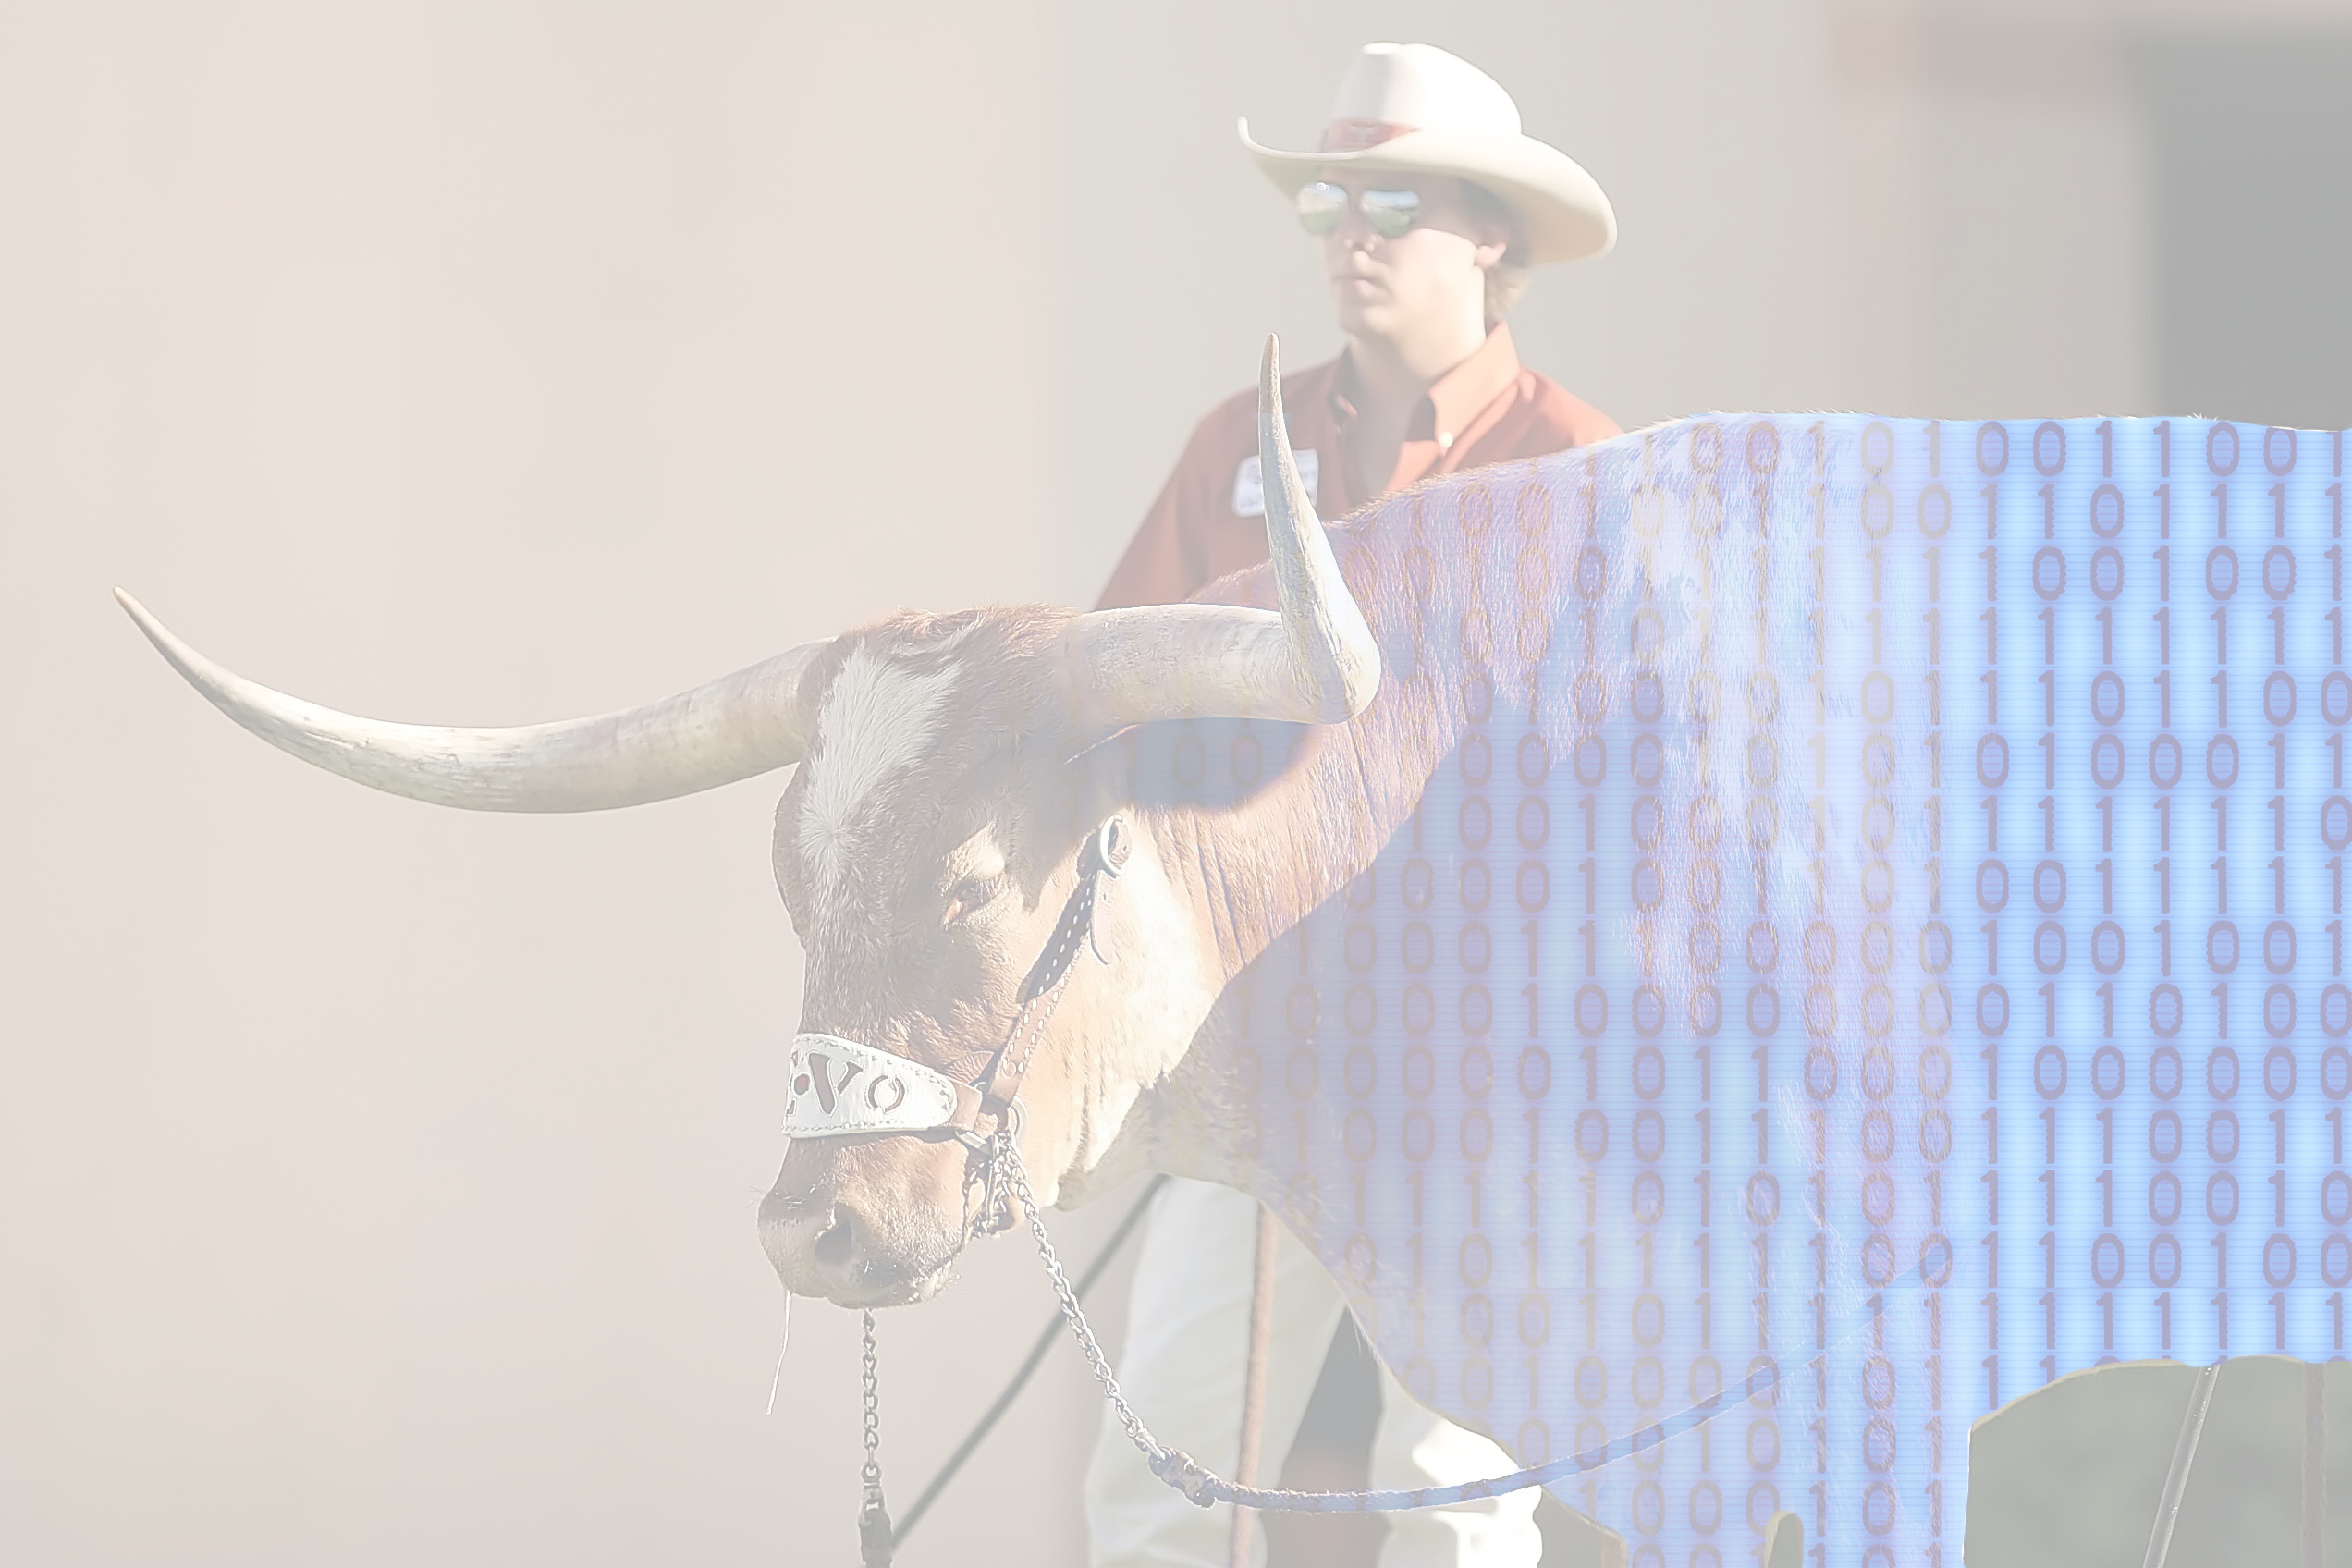
\includegraphics[height=\paperheight,keepaspectratio]{data-wrangler-BG.jpg}}
% to create image:
%   1. export data-wrangler.xcf as PNG from GIMP
%   2. convert data-wrangler.png -fill white -colorize 67% data-wrangler-BG.jpg

\begin{frame}
    \thispagestyle{empty}
    \titlepage
\end{frame}

\setbeamertemplate{background canvas}[default]


%%%%%%%%%%%%%%%%%%%%%%%%%%%%%%%%%%%%%%%%%%%%%%%%%%%%%%%%%%%%%%%%%%%%%%%%%%%%%%%%


\setbeamertemplate{background canvas}{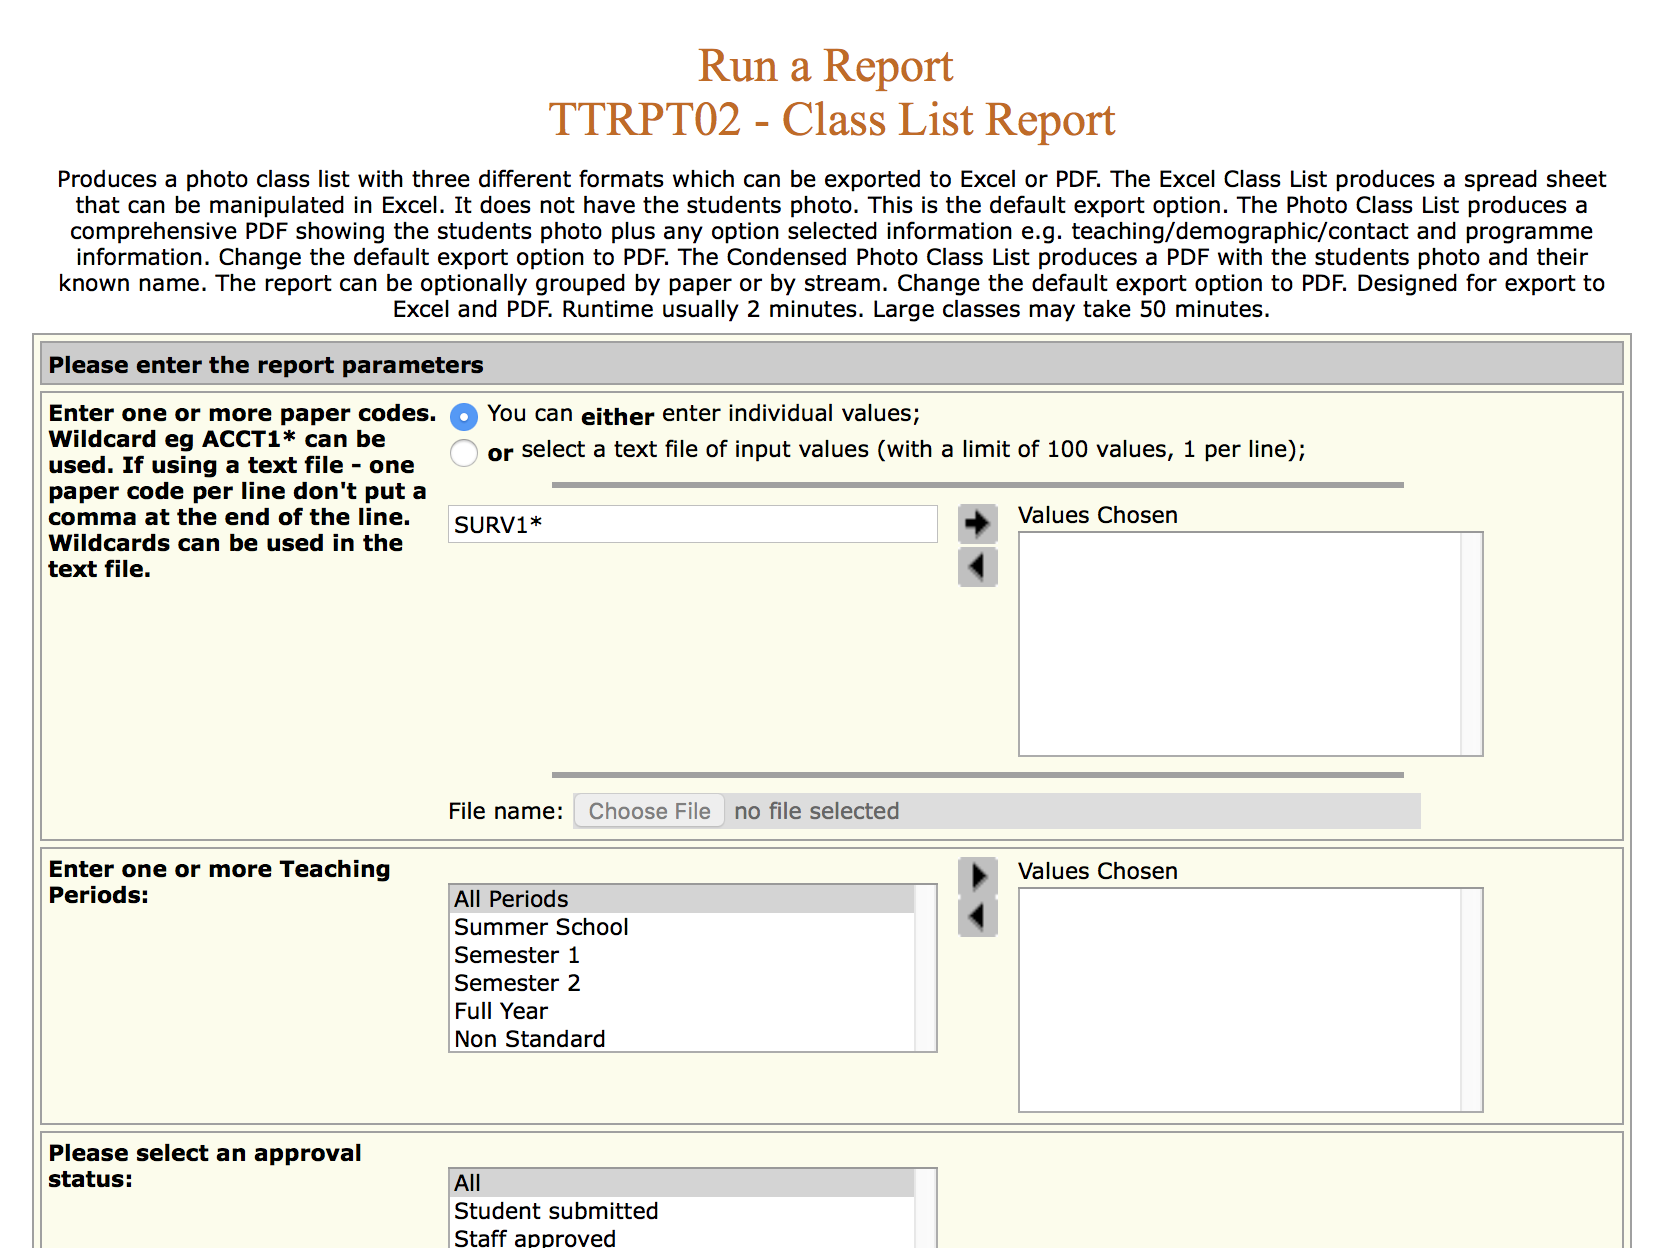
\includegraphics[width=\paperwidth,keepaspectratio]{TTRPT02.png}}

\begin{frame}
    \thispagestyle{empty}
\end{frame}

\setbeamertemplate{background canvas}[default]


%%%%%%%%%%%%%%%%%%%%%%%%%%%%%%%%%%%%%%%%%%%%%%%%%%%%%%%%%%%%%%%%%%%%%%%%%%%%%%%%


\begin{frame}
    \frametitle{Data come from a \uline{lot} of different sources}
    
    \bigskip
    \begin{columns}
        \begin{column}{0.4\paperwidth}
            \centering
            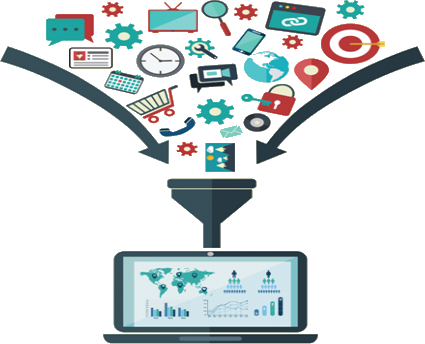
\includegraphics[width=0.9\columnwidth,keepaspectratio]{data-sources.png}\tinyskip
            {\tiny{SOURCE: Xobber}}
        \end{column}
        \begin{column}{0.55\paperwidth}
            \centering
            \begin{tabular}{cccccccc}
                \faHeartO & \faCode & \faDatabase & \faGit & \faCalendar & \faLaptop & \faThumbsOUp & \faBluetoothB \\
                \addlinespace
                \faTags & \faTerminal & \faDashboard & \faYoutubePlay & \faFileCodeO & \faLinux & \faCloud & \faBank \\
                \addlinespace
                \faBarcode & \faUsers & \faFilePdfO & \faSafari & \faAndroid & \faAmazon & \faFileAudioO & \faGavel \\
                \addlinespace
                \faFileWordO & \faFilm & \faRss & \faSteam & \faWikipediaW & \faCreditCard & \faGamepad & \faWifi \\
                \addlinespace
                \faShoppingCart & \faPaypal & \faKeyboardO & \faClockO & \faEnvelopeO & \faFileExcelO & \faTruck & \faToggleOn \\
                \addlinespace
                \faBirthdayCake & \faFolderOpenO & \faHddO & \faDesktop & \faAutomobile & \faBus & \faResistance & \faFax \\
                \addlinespace
                \faGoogle & \faFacebook & \faIndustry & \faLinkedin & \faAreaChart & \faSpotify & \faBarChart & \faFileTextO \\
                \addlinespace
                \faFloppyO & \faWeibo & \faFileArchiveO & \faFileImageO & \faPrint & \faMobile & \faApple & \faChrome \\
                \addlinespace
                \faPieChart & \faCamera & \faQrcode & \faSoccerBallO & \faMapO & \faFirefox & \faFilePowerpointO & \faEdge \\
                \addlinespace
                \faCompass & \faNewspaperO & \faFileMovieO & \faStackOverflow & \faMicrophone & \faTwitter & \faWpforms & \faPhone \\
            \end{tabular}
        \end{column}
    \end{columns}
\end{frame}


%%%%%%%%%%%%%%%%%%%%%%%%%%%%%%%%%%%%%%%%%%%%%%%%%%%%%%%%%%%%%%%%%%%%%%%%%%%%%%%%


\begin{frame}
    \frametitle{Data schemas run a wide gamut}
    
    \begin{columns}
        \begin{column}{\paperwidth}
            \centering
            \begin{tikzpicture}
                \node (erd) {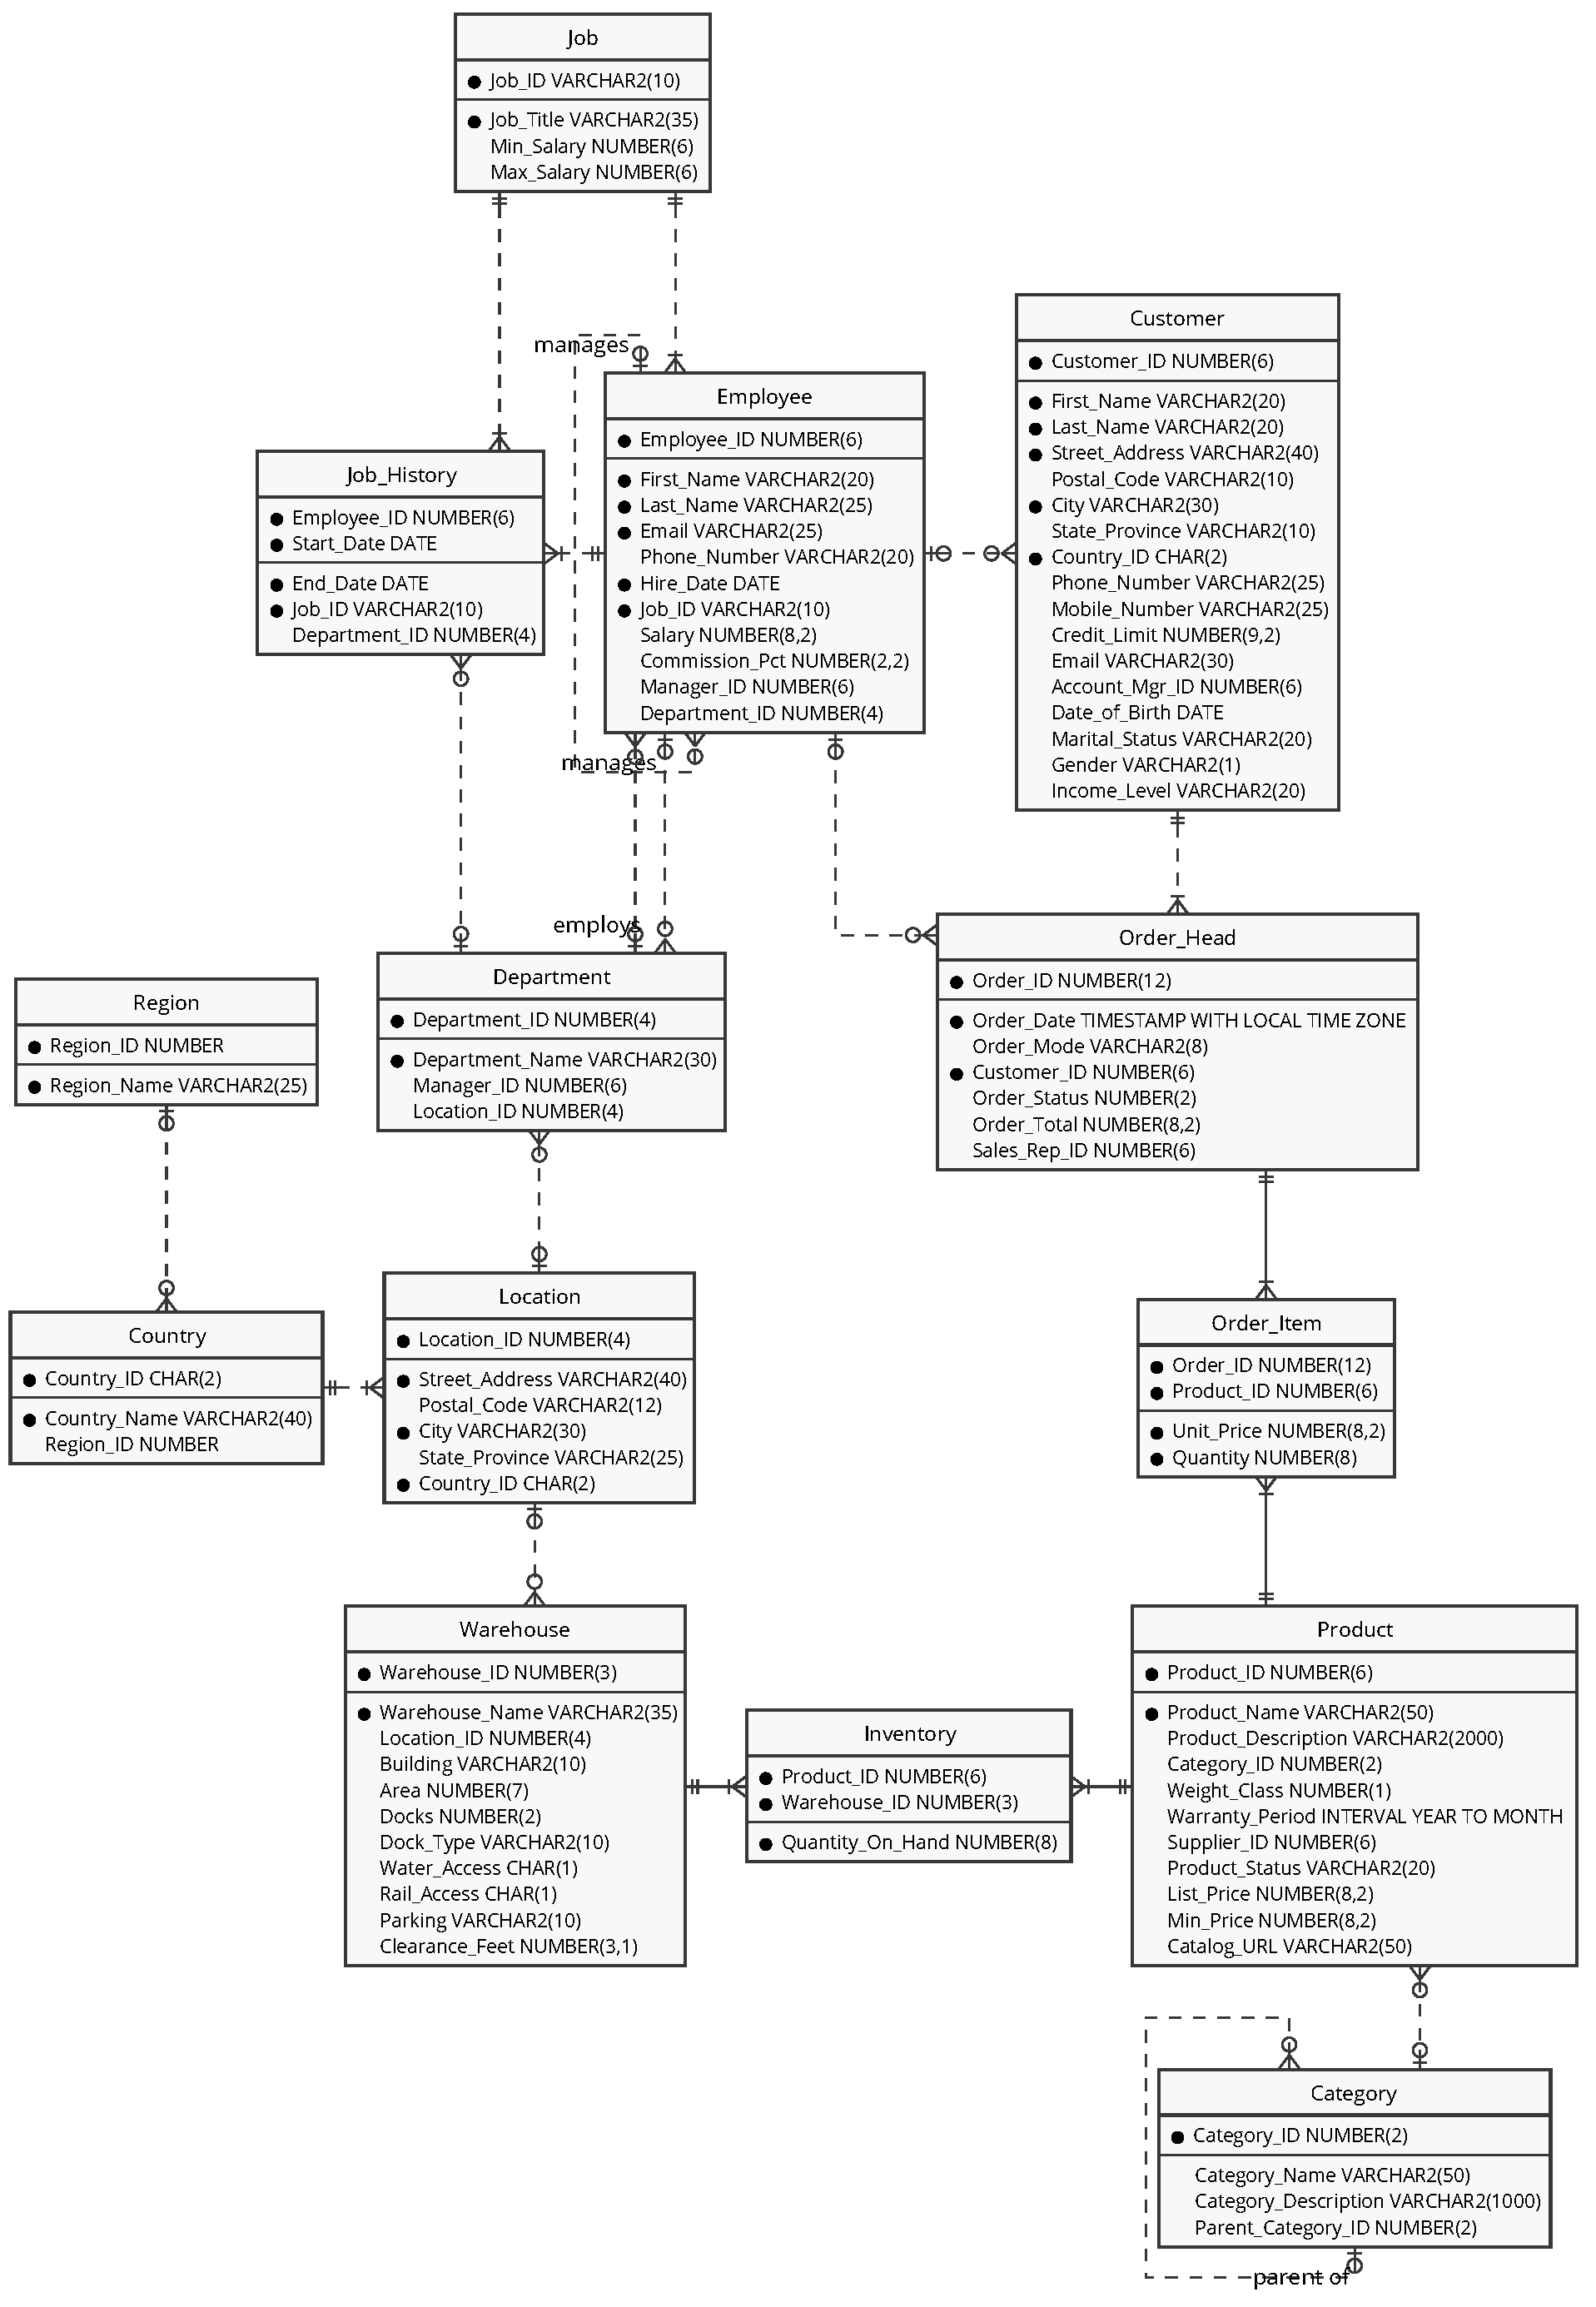
\includegraphics[width=3.25cm,keepaspectratio]{HR_OE_ERD}};
                \node[right=7.5mm of erd] (excel) {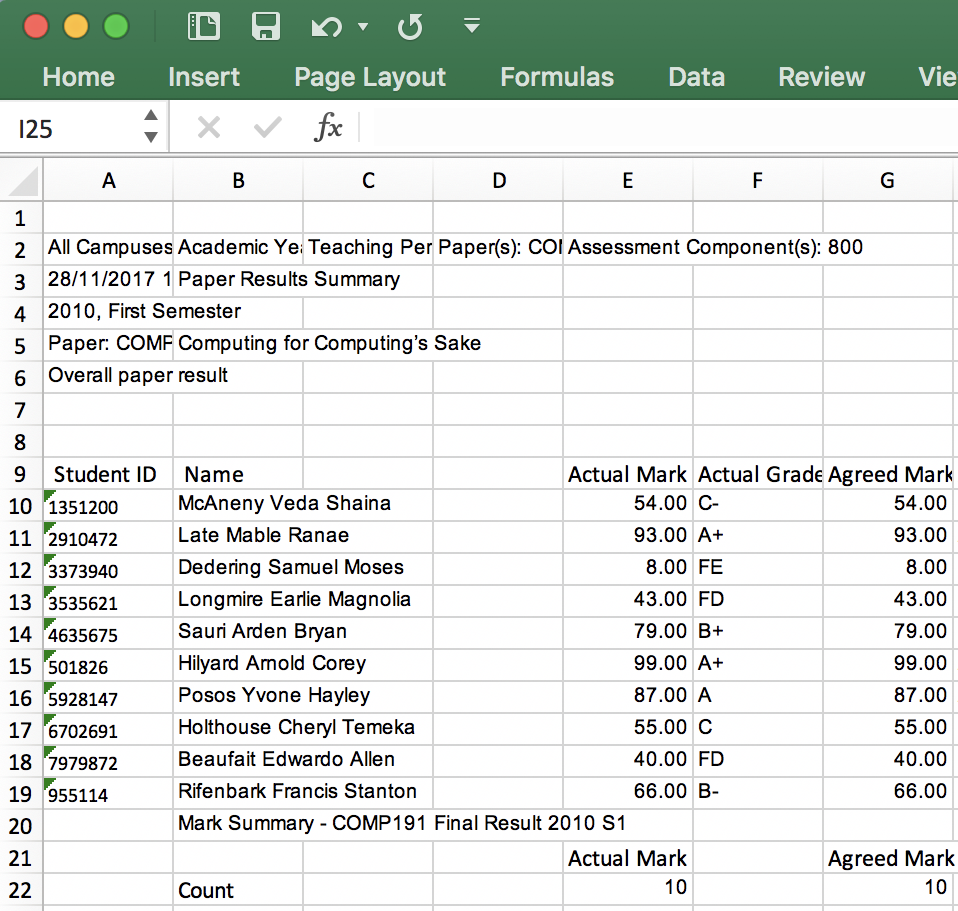
\includegraphics[width=3.25cm,keepaspectratio]{fake_results_excel}};
                \node[right=7.5mm of excel] (web) {
\includegraphics[width=3.25cm,keepaspectratio]{web_page}};
                
                \node[below=0mm of web.south] (weblabel) {free-form};
                \node (excellabel) at (excel |- weblabel) {more flexible};
                \node (erdlabel) at (erd |- weblabel) {formal, “fixed”};
                
                \node[below=-3pt of erdlabel] (erdtext) {\tiny e.g., SQL databases};
                \node[below=-3pt of excellabel] (exceltext) {\tiny e.g., JSON, XML, Excel, …};
                \node[below=-3pt of weblabel] (webtext) {\tiny e.g., email, MS Word, web pages, …};
                
                \path[fill, OU red, ultra thick, nearly transparent] (erd.west) -- ++(0,1cm) -- ($(web.west) + (0,1cm)$) -- ++(0,1cm) -- (web.east) -- ($(web.west) - (0,2cm)$) -- ++(0,1cm) -- ($(erd.west) - (0,1cm)$) -- cycle;
            \end{tikzpicture}
        \end{column}
    \end{columns}
\end{frame}


%%%%%%%%%%%%%%%%%%%%%%%%%%%%%%%%%%%%%%%%%%%%%%%%%%%%%%%%%%%%%%%%%%%%%%%%%%%%%%%%


\begin{frame}
    \frametitle{Moving data around leads to … trouble}
    
    \bigskip
    \centering
    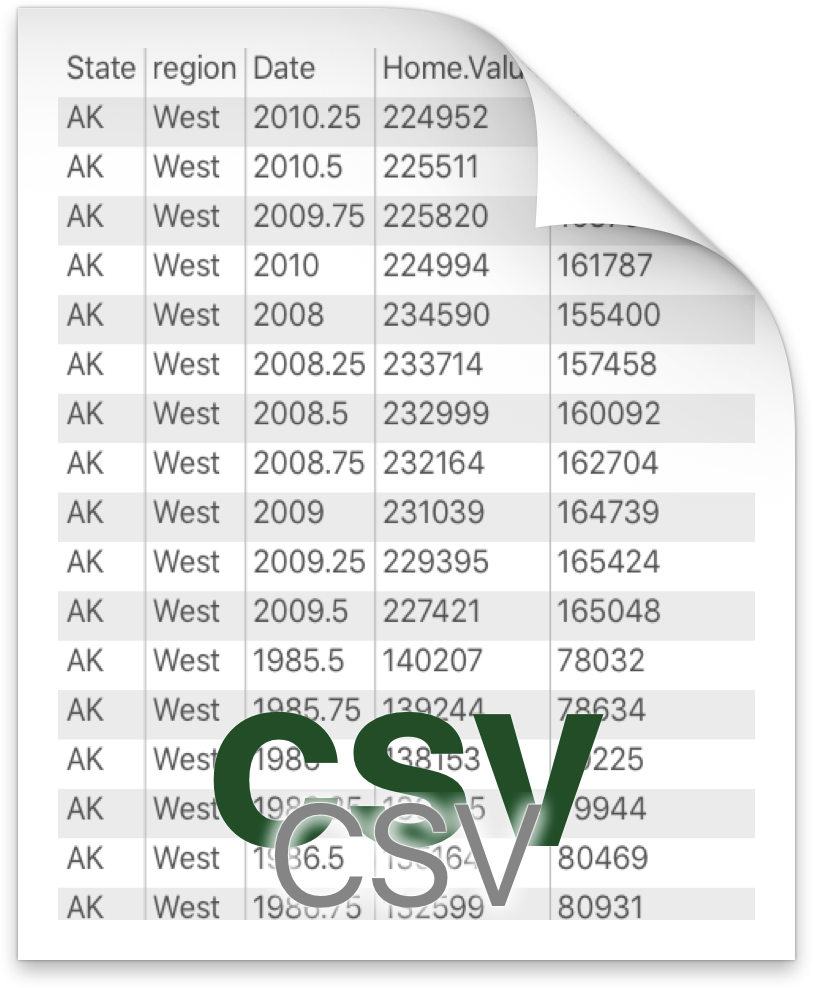
\includegraphics[height=6cm,keepaspectratio]{CSV}
\end{frame}


%%%%%%%%%%%%%%%%%%%%%%%%%%%%%%%%%%%%%%%%%%%%%%%%%%%%%%%%%%%%%%%%%%%%%%%%%%%%%%%%


\begin{frame}
    \huge
    \centering
    \bigskip\bigskip
    \structurebf{Often it’s not a case of what we can get from the data, but rather what data \emph{can} we get?}
\end{frame}


%%%%%%%%%%%%%%%%%%%%%%%%%%%%%%%%%%%%%%%%%%%%%%%%%%%%%%%%%%%%%%%%%%%%%%%%%%%%%%%%


\begin{frame}
    \frametitle{Project 1: CoreScan (completed)}
    
    \bigskip
    \begin{itemize}
        \item Statistical analysis of body composition data in R to check precision of GE’s new CoreScan algorithm.
        
        \item Data exported directly from DXA body scanner. {\tiny (dual X-ray absorptiometry)}
        
        \item Relatively straightforward:
        \begin{itemize}
            \item Excel with well-defined columns
            \item some minor cleaning
            \item trivial to automate
        \end{itemize}
        
        \item “The way things should be.”
    \end{itemize}
    
    \begin{tikzpicture}[remember picture, overlay]
        \node[above right=5mm of current page.south west)] (ref) {
            \scriptsize\parbox{\columnwidth}{Meredith-Jones, K., Haszard, J., Stanger, N., and Taylor, R. “Precision of DXA-derived visceral fat measurements in a large sample of adults of varying body size.” \emph{Obesity} \textbf{26}(3):505–512. doi:~10.1002/oby.22108}
        };
    \end{tikzpicture}
\end{frame}


%%%%%%%%%%%%%%%%%%%%%%%%%%%%%%%%%%%%%%%%%%%%%%%%%%%%%%%%%%%%%%%%%%%%%%%%%%%%%%%%


\setbeamertemplate{background canvas}{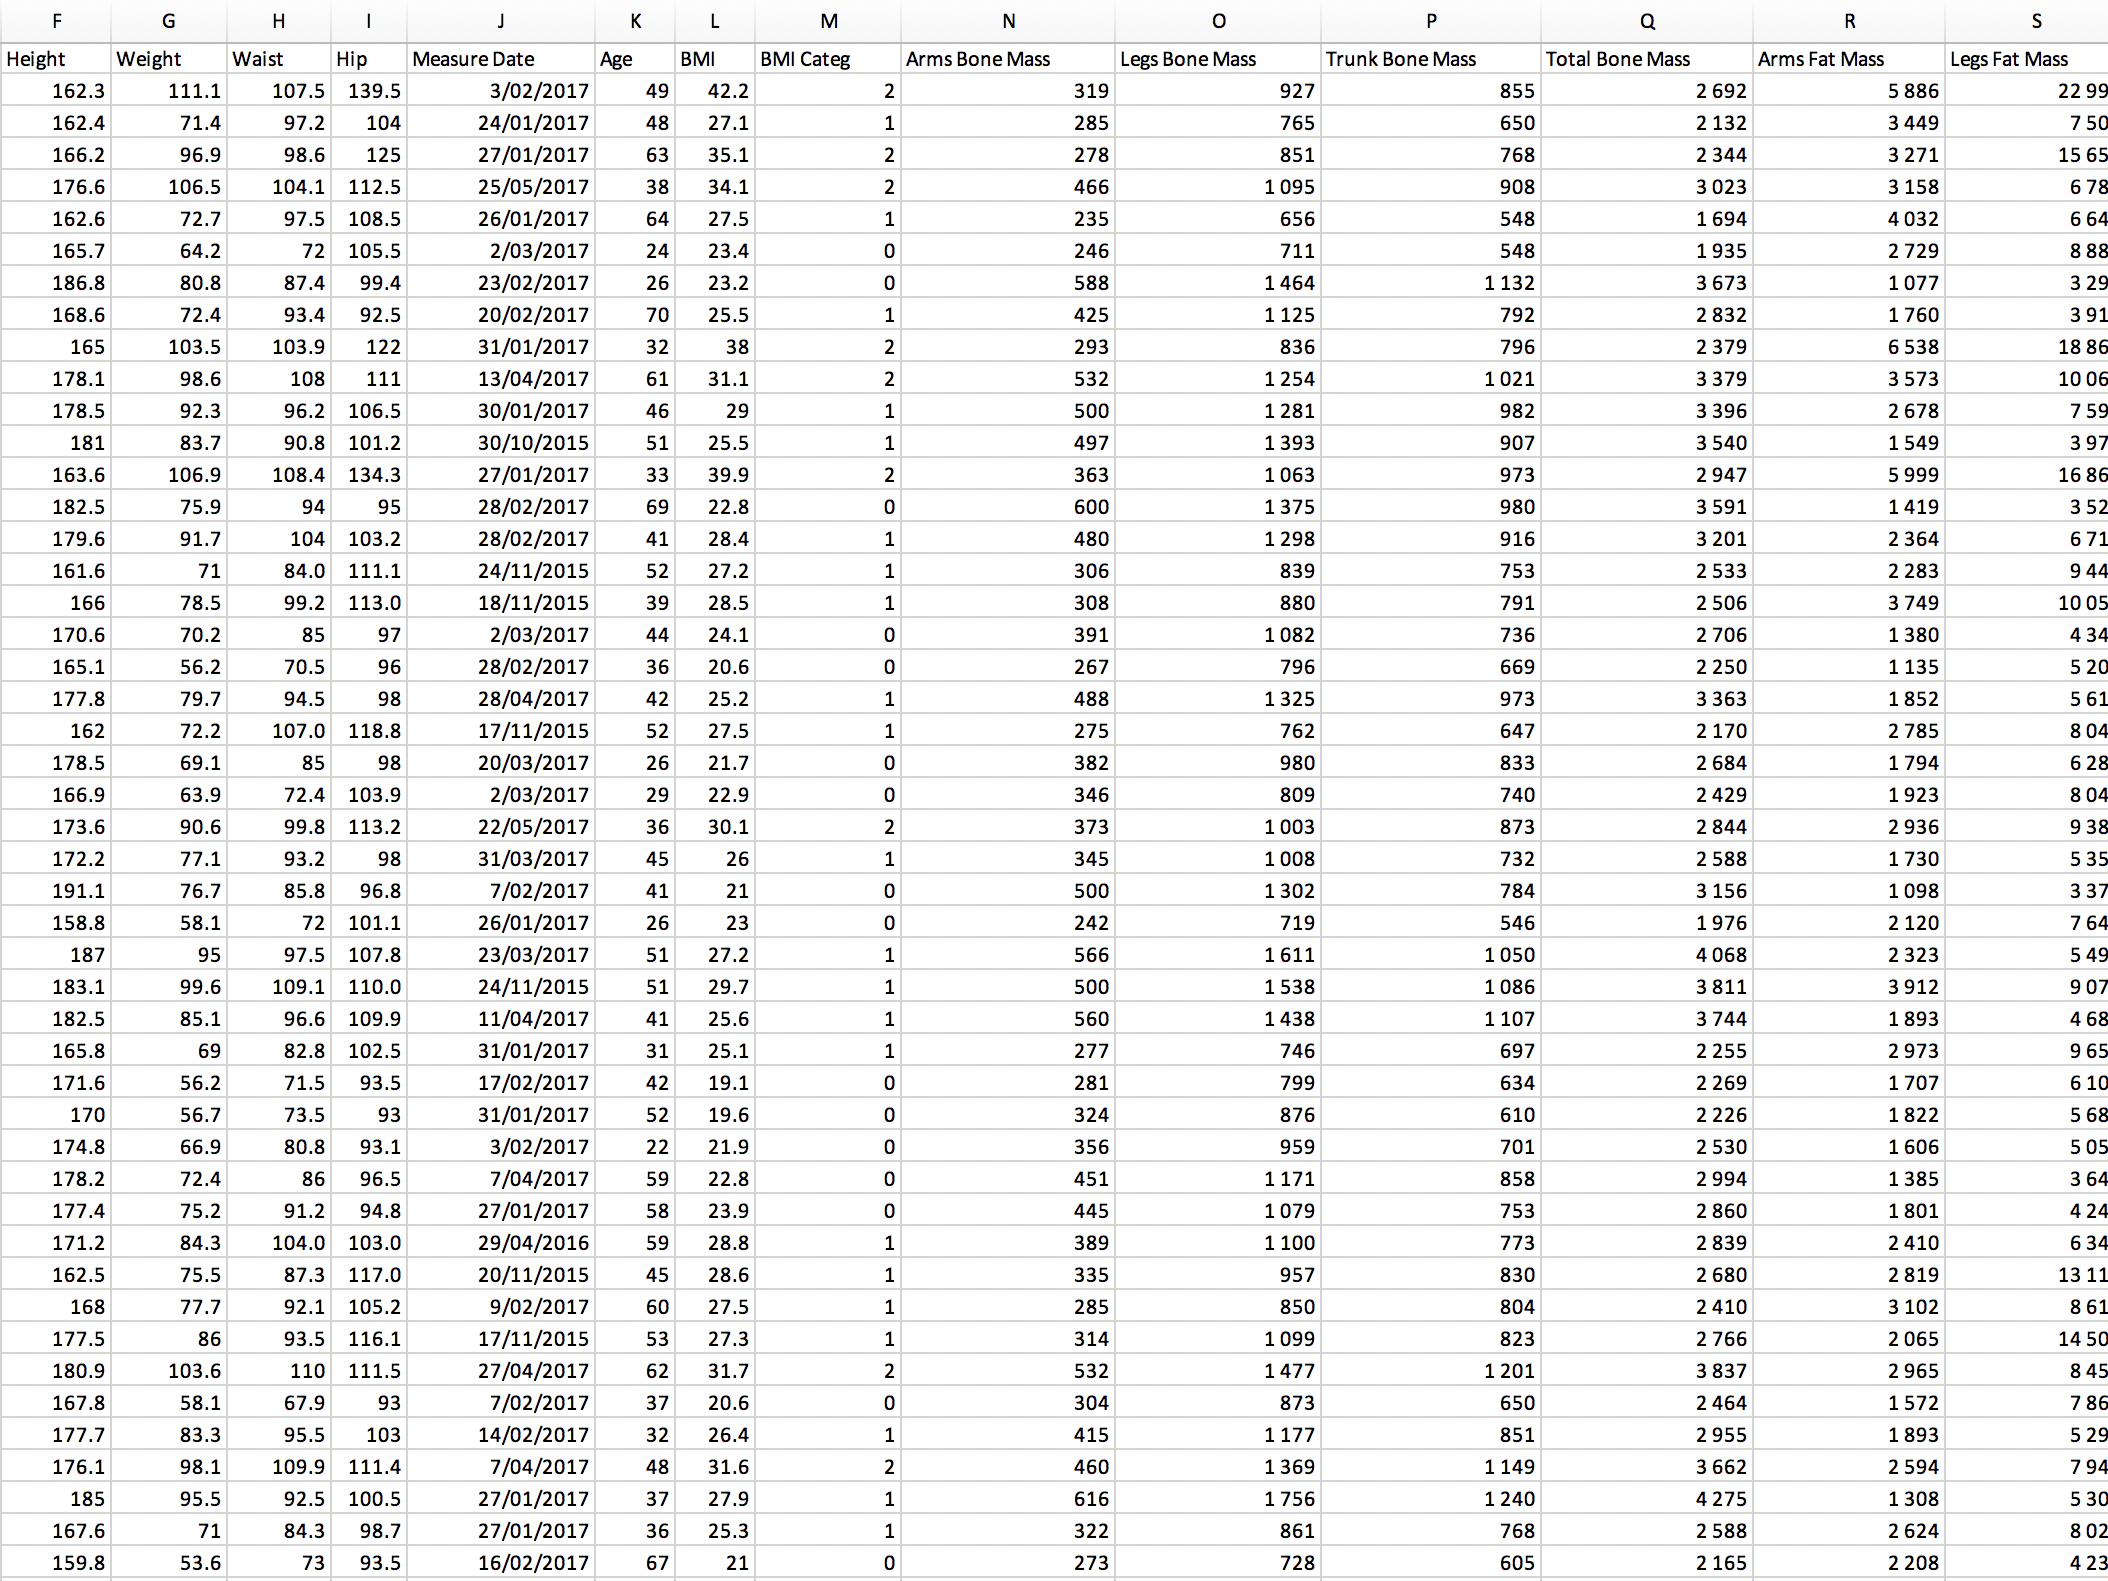
\includegraphics[width=\paperwidth,keepaspectratio]{CoreScan_data.png}}

\begin{frame}
    \thispagestyle{empty}
\end{frame}

\setbeamertemplate{background canvas}[default]


%%%%%%%%%%%%%%%%%%%%%%%%%%%%%%%%%%%%%%%%%%%%%%%%%%%%%%%%%%%%%%%%%%%%%%%%%%%%%%%%


\begin{frame}
    \frametitle{Project 2: Software licensing (barely started)}
    
    \structurebf{Which is cheaper for consumer-level software, subscription or perpetual licensing?}
    \medskip
    
    \begin{itemize}
        \item SaaS already well studied, especially for corporates.
        
        \item Typical licensing models for smaller developers:
        \begin{itemize}
            \item pay once, all updates free forever
            \item pay for each major version upgrade {\tiny (upgrade pricing)}
            \item app store (free or paid) + in-app purchases
        \end{itemize}

        \item Some are experimenting with alternative models:
        \begin{itemize}
            \item “service contract” (e.g., annual subscription)
            \item “software plus a service” (\sout{SpaS?} S+aS? S++S?)
        \end{itemize}
        
        \item Some developers offer more than one of these options.
    \end{itemize}
\end{frame}


%%%%%%%%%%%%%%%%%%%%%%%%%%%%%%%%%%%%%%%%%%%%%%%%%%%%%%%%%%%%%%%%%%%%%%%%%%%%%%%%


\begin{frame}
    \frametitle{Why do I care?}
    
    \structurebf{1Password now offers two licensing models:}
    \medskip
    
    \begin{itemize}
        \item Typical perpetual license:
        \begin{itemize}
            \item separate licenses per platform {\tiny (to enable \emph{all} features)}
            \item manually configured syncing
            \item major version upgrades are (usually) paid
        \end{itemize}
        
        \item Subscription:
        \begin{itemize}
            \item free license for all platforms
            \item transparent syncing via 1Password account
            \item annual vs.\ monthly billing
            \item individual vs.\ family
        \end{itemize}
        
        \item Both options via direct sale or app store.
    \end{itemize}
    
    \begin{tikzpicture}[remember picture, overlay]
        \node[below left=1.25cm of current page.north east)] (icon) {
            
\includegraphics[width=2cm,keepaspectratio]{1Password}
        };
    \end{tikzpicture}
\end{frame}


%%%%%%%%%%%%%%%%%%%%%%%%%%%%%%%%%%%%%%%%%%%%%%%%%%%%%%%%%%%%%%%%%%%%%%%%%%%%%%%%


\begin{frame}
    \frametitle{Cost comparison (US\$)}
    
    \begin{columns}[t]
        \begin{column}{0.45\paperwidth}
            \structurebf{“Standard” license}
            \bigskip
            
            \begin{tabular}{rrr}
                \textbf{Version}    &   \textbf{Released}   &   \textbf{Cost} \\
                2/3                 &   2009                &   \$39.95   \\
                5                   &   2014                &   \$24.99   \\
                6                   &   \todo{20??}         &   \todo{??}   \\
                7                   &   2018                &   \todo{\$39.99?}   \\
                \addlinespace
                \multicolumn{2}{r}{\textbf{Total (10 years):}}  &   \todo{??}   \\
                \multicolumn{2}{r}{\textbf{Total (per year):}}  &   \todo{??}   \\
            \end{tabular}
        \end{column}
        \begin{column}{0.45\paperwidth}
            \structurebf{Subscription}
            \begin{tabbing}
                Individual \= = \$2.99 per month \\
                \> = \$35.88 per year \\[6pt]
                Family \= = \$4.99 per month \\
                \> = \$59.88 per year
            \end{tabbing}
        \end{column}
    \end{columns}
\end{frame}


%%%%%%%%%%%%%%%%%%%%%%%%%%%%%%%%%%%%%%%%%%%%%%%%%%%%%%%%%%%%%%%%%%%%%%%%%%%%%%%%


\begin{frame}
    \frametitle{The data collection problem}
    
    \structurebf{To compare costs we need historical pricing}
    \medskip
    
    \begin{itemize}
        \item No-one’s likely to publish their pricing history! {\tiny (who cares?)}
        \begin{itemize}
            \item except maybe vendors that sell separate versions for different OS releases {\tiny (e.g. macOS Mail plugins)}
            \item at best probably only full pricing available, not upgrade
        \end{itemize}
        
        \item Wayback Machine? {\tiny (Internet Archive)}
        \begin{itemize}
            \item have successfully found a couple of old store-fronts
            \item probably impossible to automate \faFrownO
        \end{itemize}
        
        \item Trivial to process, but effectively worst case to acquire.
        
        \item Watch this space!
    \end{itemize}
\end{frame}


%%%%%%%%%%%%%%%%%%%%%%%%%%%%%%%%%%%%%%%%%%%%%%%%%%%%%%%%%%%%%%%%%%%%%%%%%%%%%%%%


\begin{frame}
    \frametitle{“Project” 3: Student data (ongoing)}
    
    \begin{itemize}
        \item For teaching \& administration:
        \begin{itemize}
            \item class lists, email lists
            \item timetabling \& streaming
            \item internal assessment, terms, final results {\tiny (processing \& submission)}
        \end{itemize}
        
        \item For research:
        \begin{itemize}
            \item CALT project on data driven course advising
            \item efficacy of teaching/tool interventions
            \item …
        \end{itemize}
    \end{itemize}
\end{frame}


%%%%%%%%%%%%%%%%%%%%%%%%%%%%%%%%%%%%%%%%%%%%%%%%%%%%%%%%%%%%%%%%%%%%%%%%%%%%%%%%


\begin{frame}
    \frametitle{Data driven course advising}
    
    \begin{itemize}
        \item For teaching \& administration:
        \begin{itemize}
            \item class lists, email lists
            \item internal assessment, terms
            \item timetabling
            \item \alert<2>{final results {\tiny (INFORMS)}}
        \end{itemize}
        
        \item For research:
        \begin{itemize}
            \item \alert<2>{CALT project on data driven course advising {\tiny (UCAN)}}
            \item efficacy of teaching/tool interventions
        \end{itemize}
    \end{itemize}
\end{frame}


%%%%%%%%%%%%%%%%%%%%%%%%%%%%%%%%%%%%%%%%%%%%%%%%%%%%%%%%%%%%%%%%%%%%%%%%%%%%%%%%


\begin{frame}
    \frametitle{INFORMS}
    
    \begin{itemize}
        \item Started as PostgreSQL database + tools to automate results files for Student Records. {\tiny (ca.\ 2001–2002)}
        
        \item Has grown “organically”:
        \begin{itemize}
            \item transforming data to and from central systems {\tiny (pre and post eVision)}
            \item level of award calculation
            \item grade histograms
            \item web interface for some functions
            \item[\faArrowRight] a mishmash of bash, Perl, Python, PHP, R, AppleScript (!), iMacros, HTML, CSS, JavaScript
        \end{itemize}
    \end{itemize}
    \bigskip\bigskip\bigskip\mbox{}
    
    \begin{tikzpicture}[remember picture, overlay]
        \node[anchor=south west, above right=2mm of current page.south west] (home) {
            
\includegraphics[height=3cm,keepaspectratio]{INFORMS_home}
        };
        \node[anchor=south east, above left=2mm of current page.south east] (files) {
            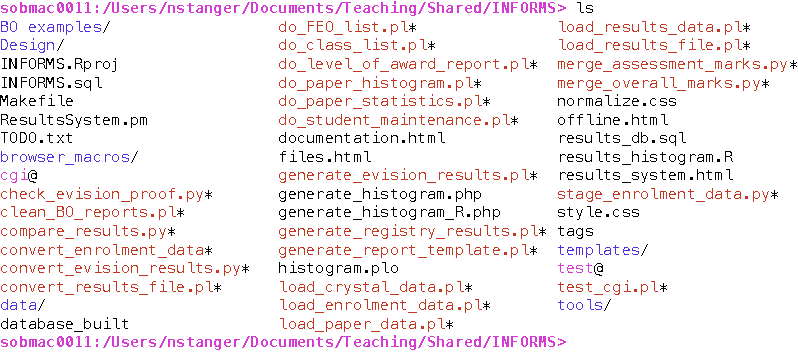
\includegraphics[height=3cm,keepaspectratio]{INFORMS_files}
        };
    \end{tikzpicture}
\end{frame}


%%%%%%%%%%%%%%%%%%%%%%%%%%%%%%%%%%%%%%%%%%%%%%%%%%%%%%%%%%%%%%%%%%%%%%%%%%%%%%%%


\begin{frame}
    \frametitle{Data driven course advising}
    \framesubtitle{(with Sander, Claudia, Steven)}
    
    \begin{itemize}
        \item CALT project looking at evidence-based approaches to improve course advising. {\tiny (among others)}
        
        \item Under way for about 7 months.
        
        \item Needs a lot of historical student data.
        \begin{itemize}
            \item enrolments, results, student performance, workload, completion, demographics, …
            \item initially focused on COSC and INFO papers only
        \end{itemize}
        
        \item Currently using a modified version of INFORMS database.
    \end{itemize}
\end{frame}


%%%%%%%%%%%%%%%%%%%%%%%%%%%%%%%%%%%%%%%%%%%%%%%%%%%%%%%%%%%%%%%%%%%%%%%%%%%%%%%%


\begin{frame}
    \frametitle{Data sources}
    
    \begin{tikzpicture}[remember picture, overlay]
        \node[anchor=south east, above left=4mm of current page.south east] (ttrpt02) {
            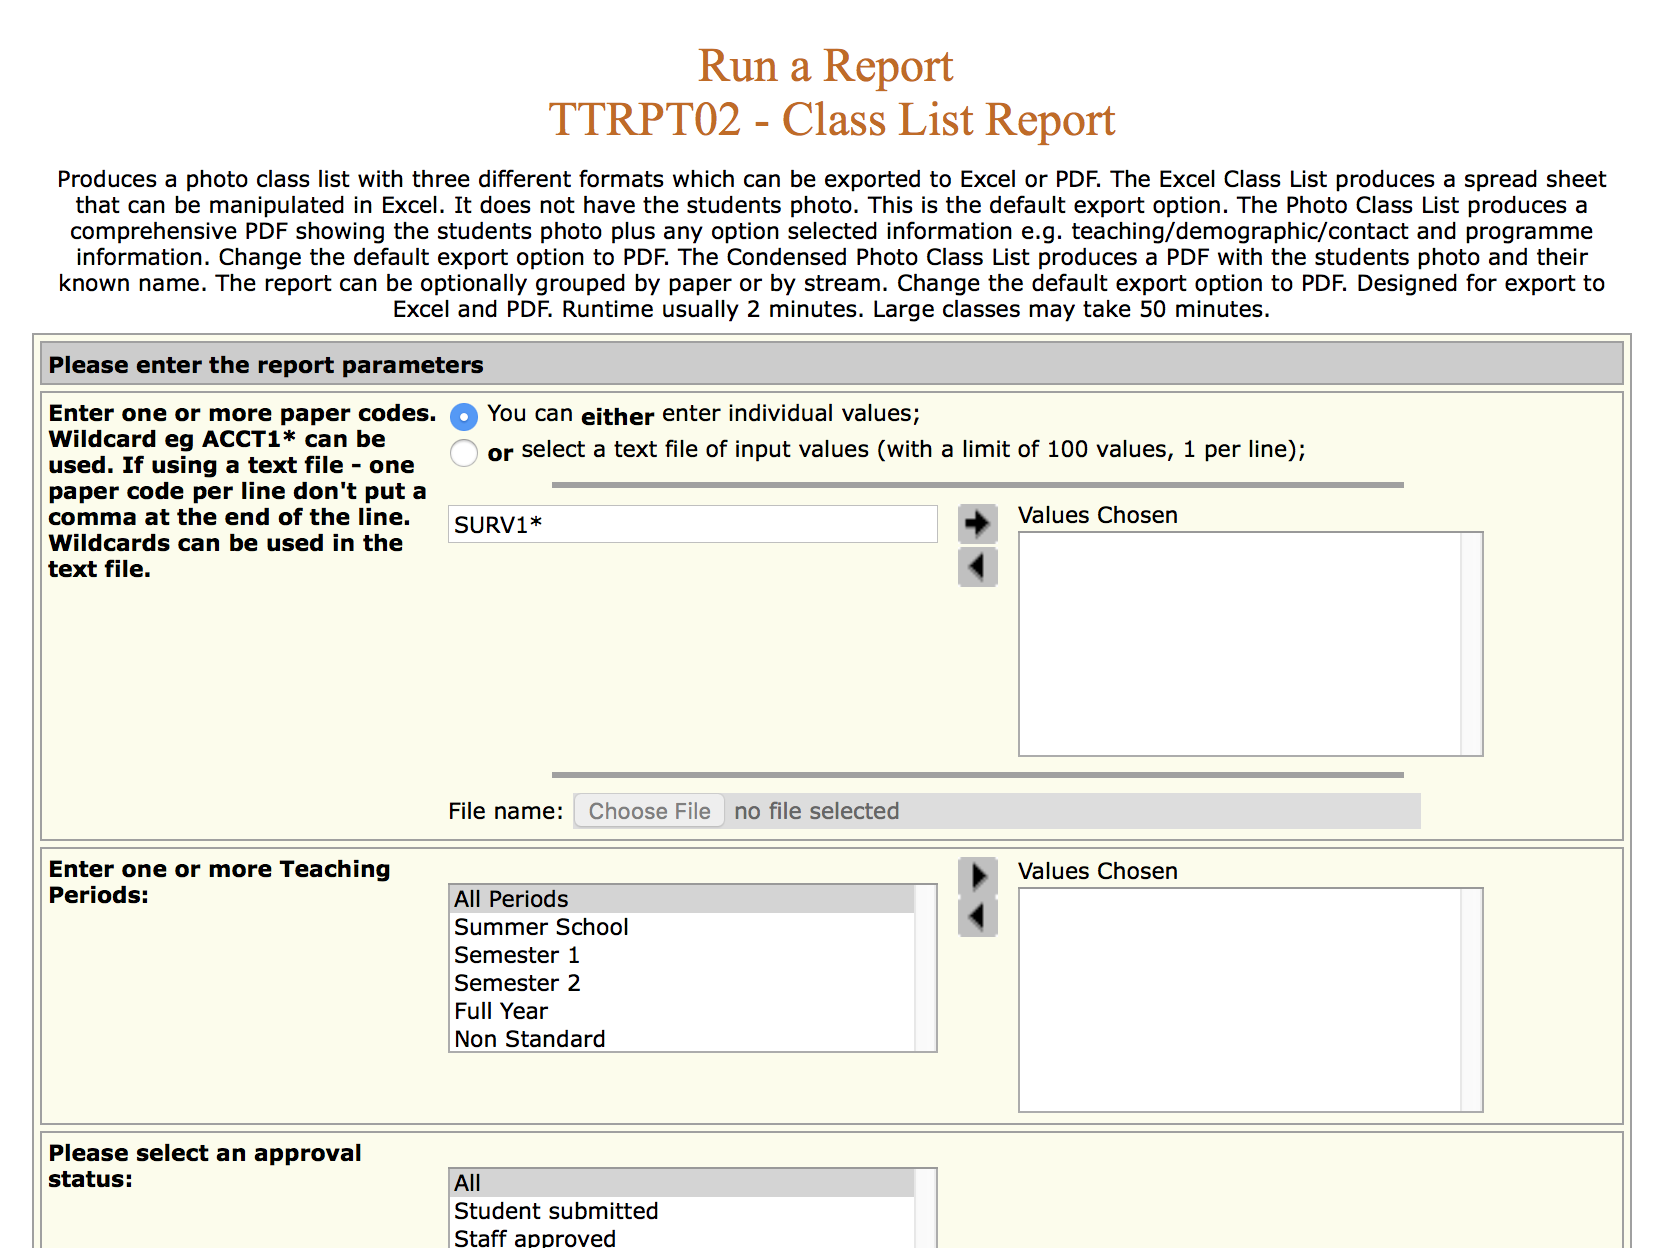
\includegraphics[height=2.8cm,keepaspectratio]{TTRPT02.png}
        };
    \end{tikzpicture}
    
    \begin{itemize}
        \item Mostly eVision via Business Objects. {\tiny (maybe Blackboard for internal assessment)}
        \begin{itemize}
            \item human readable (PDF \faFilePdfO, Word \faFileWordO)
            \item “machine-readable” (CSV \faFileTextO, XLS \faFileExcelO)
        \end{itemize}
    \end{itemize}
    \medskip
    
    \begin{tabular}{lp{8cm}}
        \structurebf{CARPT004}  &   Paper, student, and enrolment data  \\
        \structurebf{TTRPT02}   &   Enrolment and streaming data  \\
        \structurebf{EXRPT11}   &   Final results and internal assessment {\tiny (Results I vs.\ II)}  \\
        \structurebf{SDRPT12}   &   Student retention, including degree completion and annual workload  \\
        \structurebf{SDGPA01}   &   GPA data (per year, level,  \\
                                &   and overall)  \\
    \end{tabular}
\end{frame}


%%%%%%%%%%%%%%%%%%%%%%%%%%%%%%%%%%%%%%%%%%%%%%%%%%%%%%%%%%%%%%%%%%%%%%%%%%%%%%%%


\begin{frame}
    \frametitle{Typical problems encountered}
    
    \begin{itemize}
        \item Old formats (.xls) \(\Rightarrow\) long term preservation issues.
        
        \item Business Objects reports were developed “organically”:
        \begin{itemize}
            \item inconsistent parameters
            \item ad hoc design
            \item more likely to be designed for human readability
            \item can change without warning {\tiny (esp.\ after eVision rollout)}
        \end{itemize}
        
        \item No API access \(\Rightarrow\) no ad hoc querying.
        
        \item Reading delimited text is often easier. \faMehO
    \end{itemize}
\end{frame}


%%%%%%%%%%%%%%%%%%%%%%%%%%%%%%%%%%%%%%%%%%%%%%%%%%%%%%%%%%%%%%%%%%%%%%%%%%%%%%%%


\begin{frame}
    \frametitle{EXRPT11 “Tabular” report}
    
    \bigskip
    Stated as “must run in Excel” \(\Rightarrow\) intended to be \alert{machine readable}.
    \bigskip
    
    \centering
    \begin{tikzpicture}
        \node[anchor=south west] (ss) {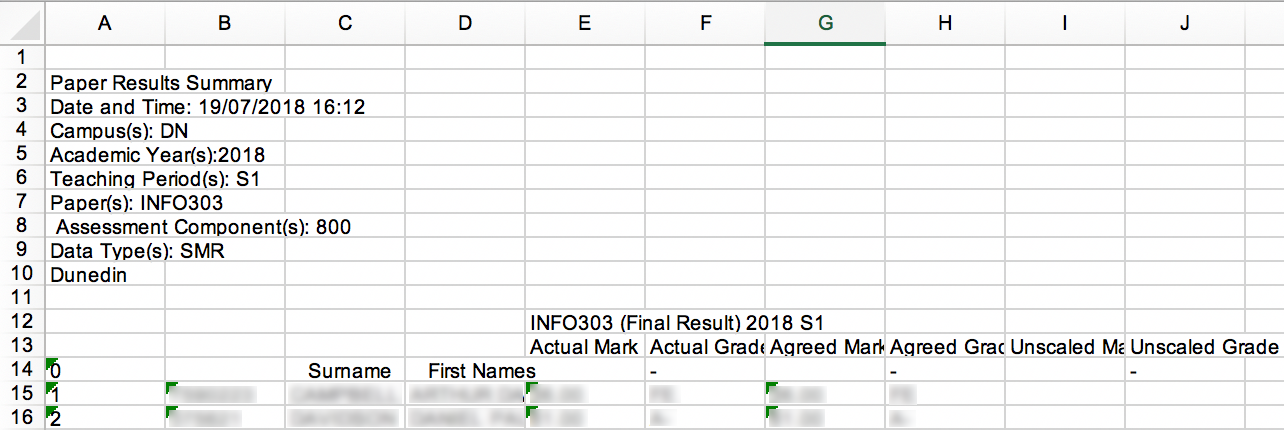
\includegraphics[width=0.95\columnwidth,keepaspectratio]{EXRPT11_Tabular}};
        \begin{uncoverenv}<2>
            \node[draw, ultra thick, ellipse, OU red, minimum width=1cm] (id) at (1.9cm,0.6cm) {};
            \node[draw, ultra thick, ellipse, OU red, minimum width=3cm, minimum height=0.7cm] (grades) at (5.8cm,0.7cm) {};
            \node[OU red] (wtf) at (3.5cm,-0.8cm) {\textbf{?!?!}};
            \draw[OU red, thick, -{Stealth}] (wtf) -- (id);
            \draw[OU red, thick, -{Stealth}] (wtf) -- (grades);
        \end{uncoverenv}
    \end{tikzpicture}
\end{frame}


%%%%%%%%%%%%%%%%%%%%%%%%%%%%%%%%%%%%%%%%%%%%%%%%%%%%%%%%%%%%%%%%%%%%%%%%%%%%%%%%


\begin{frame}
    \frametitle{EXRPT11 “Summary” report}
    
    \bigskip
    Stated as “must run in PDF” \(\Rightarrow\) \alert{not} intended to be machine readable.
    \bigskip
    
    \centering
    \begin{tikzpicture}
        \node (ss) {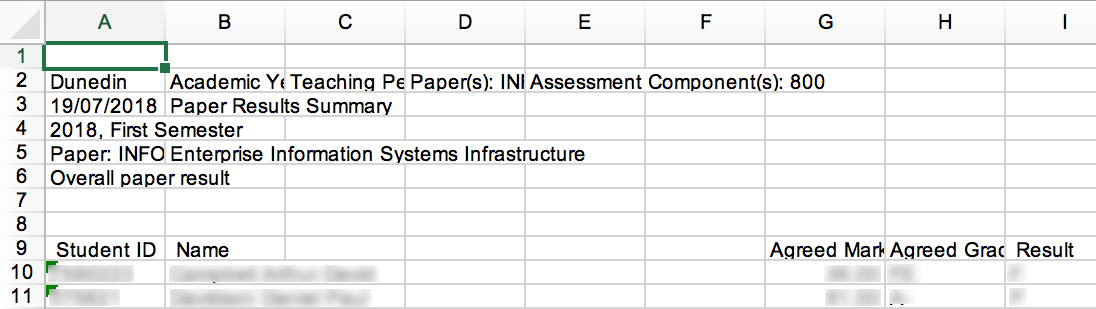
\includegraphics[width=0.95\columnwidth,keepaspectratio]{EXRPT11_Summary}};
        \node[OU red, below=5mm of ss] (huh) {\huge\textbf{!!!}};
    \end{tikzpicture}
\end{frame}


%%%%%%%%%%%%%%%%%%%%%%%%%%%%%%%%%%%%%%%%%%%%%%%%%%%%%%%%%%%%%%%%%%%%%%%%%%%%%%%%


\begin{frame}
    \frametitle{SDRPT12 mysteriously fixed itself}
    
    \bigskip
    \structurebf{\alt<2>{July 2018}{Early 2018}}
    \bigskip
    
    \centering
    \begin{tikzpicture}
        \node (broken) {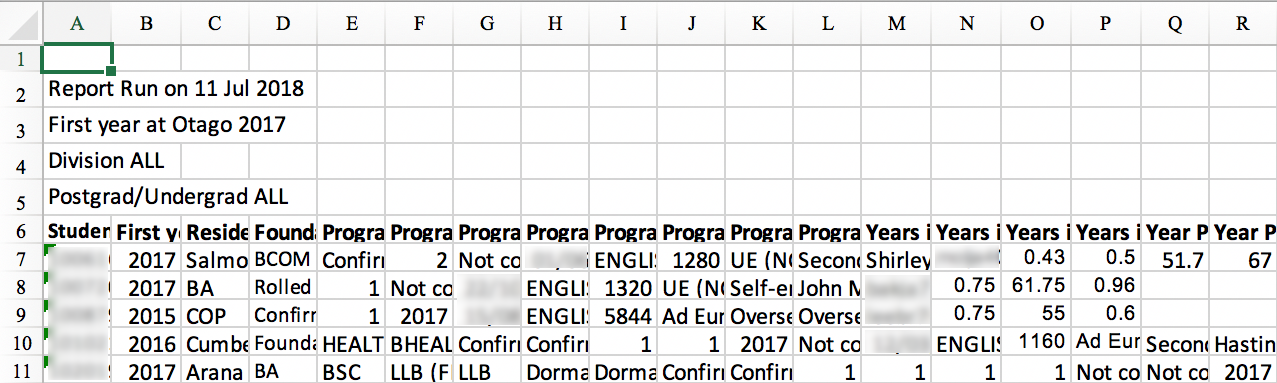
\includegraphics[width=0.95\columnwidth,keepaspectratio]{SDRPT12_bustificated}};
        \uncover<2>{\node (fixed) {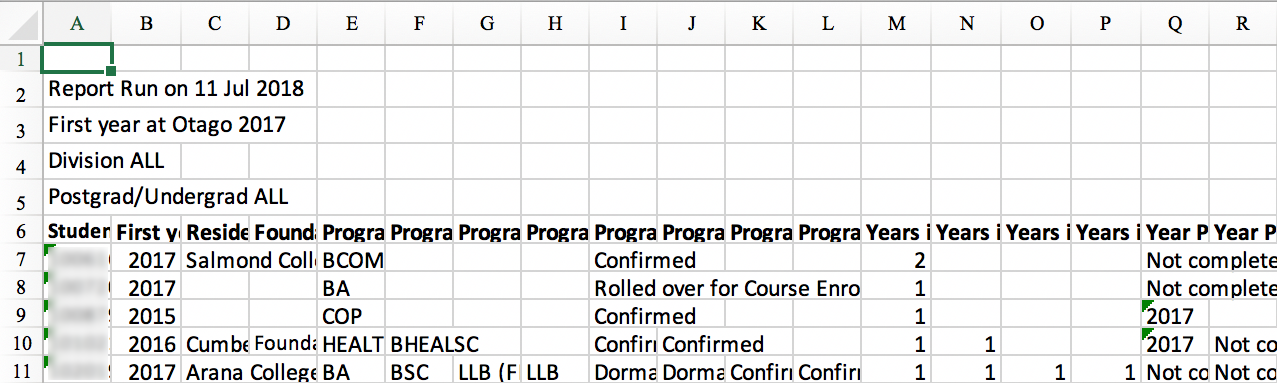
\includegraphics[width=0.95\columnwidth,keepaspectratio]{SDRPT12_fixed}};}
    \end{tikzpicture}
    \bigskip
    
    \footnotesize
    \uncover<2>{(This is good, as the only other source of completion data is the student transcript.)}
\end{frame}


%%%%%%%%%%%%%%%%%%%%%%%%%%%%%%%%%%%%%%%%%%%%%%%%%%%%%%%%%%%%%%%%%%%%%%%%%%%%%%%%


\begin{frame}
    \centering\Huge
    \structurebf{Questions?}
\end{frame}


%%%%%%%%%%%%%%%%%%%%%%%%%%%%%%%%%%%%%%%%%%%%%%%%%%%%%%%%%%%%%%%%%%%%%%%%%%%%%%%%


\end{document}

Project 2: student data
• CALT project about data-driven course advising
    • one potential output is a tool that illustrates student progression (show medical animation example)
    • needs enrolment data in a graph form (each node represents a paper and each edge represent a transition between papers)
• where do these data come from?
    • perhaps Blackboard if you’re using that for internals
        • exports as “.xls.csv” (!)
    • CARPT004 for some enrolment data
    • TTRPT02 for remaining enrolment data not already in CARPT004 and TTRPT02 (find out what each provides)
    • recent development: LDAP for creating class email lists



Why are things still like this?
• lack of demand/knowledge/education on the part of data consumers (“you get that with computers”) — don’t realise things could be much better
    • e.g., Heather’s three pages of instructions vs. Mark’s quick and dirty VBA app for generating class email lists
• apathy/lack of response from data providers (e.g., ITS)
    • “we’ll do it if you pay for it”
    • “why would you need that?”
    • “we can’t open up our systems like that — too risky”
    • focused on bigger projects/needs?
• apathy on the part of consumers who do know better
    • usually because they already have workarounds that are “good enough”
• ancient software/interfaces (e.g., Business Objects)

